% !Mode:: "TeX:UTF-8"
% VL 14, gebaut aus part-architekturen-anwendungen/23-latente-raeume.md und
% 24-anwendungsbeispiele.md (ohne Vibecoding, das kommt in VL 15).
% (Dialogmuster und Zeiten: transcripts/vl13-latent-spaces-anwendungen-2025/notiz.md).
% !Mode:: "TeX:UTF-8"
\newcommand{\thepage}{} % to silence a hyperref warning about pdfpagelabels
\RequirePackage[]{silence}
\WarningsOff[hyperref]
\PassOptionsToPackage{log-declarations=false}{xparse}
%\RequirePackage[l2tabu, orthodox]{nag}
\RequirePackage{luatex85} % to make \pdf...= commands work with LuaTeX
\documentclass[aspectratio=169,t]{beamer}
\usepackage{ifthen}
\usepackage[T1]{fontenc}
\usepackage{iftex}
\ifLuaTeX
 \usepackage{fontspec}
 \setmainfont[Ligatures=TeX]{Source Sans Pro}
\else
 \usepackage[utf8]{inputenc}
\fi
\usepackage{german}
\usepackage{newunicodechar}
\newunicodechar{€}{\texteuro}
\newunicodechar{ß}{\ss}
\renewcommand{\SS}{\iffontchar\font"1E9E \symbol{"1E9E}\else SS\fi}
\usepackage{ellipsis}
\usepackage{microtype}
\usepackage{listings}
\usepackage{sourcecodepro}
\lstset{language=Python, basicstyle=\ttfamily}
\usepackage{amsfonts}
\usepackage{amssymb}
\usepackage{amsthm}
\usepackage{fancyhdr}
\usepackage{graphicx}

\newtheorem{proposition}[theorem]{Proposition}

\DeclareMathOperator*{\argmax}{argmax}
\DeclareMathOperator{\supp}{supp}
\newcommand{\E}{\ensuremath{\mathbb{E}}}
\newcommand{\V}{\ensuremath{\mathbb{V}}}

\setbeamercolor{emph}{fg=purple}
\renewcommand<>{\emph}[1]{%
  {\usebeamercolor[fg]{emph}\only#2{\itshape}#1}%
}



\hypersetup{draft=false,colorlinks=false,pdfpagemode=UseOutlines,plainpages=false,
            breaklinks=true,bookmarksnumbered=true,pdfborder=0 0 0,
            pdftitle={Einführung in Deep Learning WiSe 2026/27 HHU},
            pdfauthor={Konrad Voelkel},
            pdfsubject={data science}}

%\documentclass[aspectratio=169,t]{beamer}
\usetheme{hhubeamer} % put the hhu-beamer-theme in /usr/share/texmf/tex/latex/beamer/themes/

% -------------------- Code listings config --------------------
% Define custom colors for syntax highlighting
\definecolor{codegreen}{rgb}{0,0.6,0}
\definecolor{codegray}{rgb}{0.5,0.5,0.5}
\definecolor{codepurple}{rgb}{0.58,0,0.82}
\definecolor{backcolour}{rgb}{0.96,0.96,0.94} % Very light gray/beige
% Configure the listings package
\lstset{
    language=Python,
    backgroundcolor=\color{backcolour},   
    commentstyle=\color{codegreen}\itshape,
    keywordstyle=\color{blue}\bfseries,
    numberstyle=\tiny\color{codegray},
    stringstyle=\color{codepurple},
    basicstyle=\ttfamily\footnotesize, % Use a monospaced font
    breakatwhitespace=false,         
    breaklines=true,      
             % Enable automatic line breaking
    captionpos=b,                      % Caption at the bottom
    keepspaces=true,                 
    numbers=left,                      % Line numbers on the left
    numbersep=10pt,                    % Distance of line numbers from the code
    showspaces=false,                
    showstringspaces=false,            % Don't show weird underscores in strings
    showtabs=false,                  
    tabsize=4,
    frame=single,                      % Add a subtle border around the code
    rulecolor=\color{black!20},        % Border color
  }

\event[]{}
\author[Wintersemester 2026/27]{Dr. Konrad Völkel, Wintersemester 2026/27}

%\title{Data Science, VL 1}
%\date{16.04.2026}


%%% Local Variables:
%%% mode: latex
%%% TeX-master: t
%%% End:


% Fassung mit Dozentennotizen (zweiter Schirm): die nächste Zeile einkommentieren.
% \setbeameroption{show notes on second screen=right}

\graphicspath{{../images/}}

\title[Latente Räume (VL 14)]{Latente Räume und Anwendungen\\\large Einführung in Deep Learning, VL 14}
\date{27.01.2027}

\begin{document}

\begin{frame}
  \titlepage

  \note{\textbf{Ablauf, 90 Minuten} (2025: 51 Min. latente Räume, 33 Min. Anwendungen als
    Dialog):\\[2pt]
    \begin{tabular}{@{}rll@{}}
      0--4   & Folie 2       & Probeklausur ist abgegeben\\
      4--16  & Folien 3--5   & Arithmetik im latenten Raum, Bias\\
      16--26 & Folien 6--7   & Interpolation, Superposition\\
      26--40 & Folien 8--10  & Diskret dekodieren: top-$k$, Temperatur\\
      40--52 & Folien 11--13 & Bilder: AE, VAE, GAN im Vergleich\\
      52--60 & Folie 14      & Latent Space Oddity\\
      60--84 & Folien 15--18 & \textbf{Anwendungsbeispiele als Dialog}\\
      84--90 & Folie 19      & Das Rezept, Klausurhinweis\\
    \end{tabular}\\[4pt]
    \textbf{Der Anwendungsteil ist ein Dialog}, kein Vortrag: Der Hörsaal schlägt jeden
    Schritt vor, die Folie bestätigt. 2025 hat allein hAInrich 26 Minuten getragen.}
\end{frame}

\begin{frame}
  \frametitle{Wo wir stehen}

  \begin{center}
    \Large
    Autoencoder, VAE, word2vec, GAN --\\
    alle haben einen latenten Raum.\\[16pt]
    Heute: Was ist das eigentlich für ein Raum?
  \end{center}

  \note{Die Probeklausur ist heute abgegeben, Besprechung in der Übung morgen.
    Heute keine neue Architektur, sondern ein zweiter Blick auf alles, was wir gebaut
    haben.}
\end{frame}

\begin{frame}
  \frametitle{Arithmetik im latenten Raum}

  \begin{center}
    \Huge KING $-$ MAN $+$ WOMAN $=$ QUEEN
  \end{center}

  \note{Der Klassiker bei word2vec. Also ist WOMAN $-$ MAN die Richtung „feminin“.
    Weitere: PARIS $-$ FRANCE $+$ ITALY $=$ ROME (Richtung „Hauptstadt“),
    WALKING $-$ WALK $+$ SWIMMING $=$ SWAM (Richtung „Vergangenheit“).
    \textbf{Die eigentliche Pointe:} Darauf wurde nicht trainiert. Das entsteht von selbst
    aus dem Kontext-Vorhersage-Training.}
\end{frame}

\begin{frame}
  \frametitle{Richtungen bedeuten etwas}

  \begin{center}
    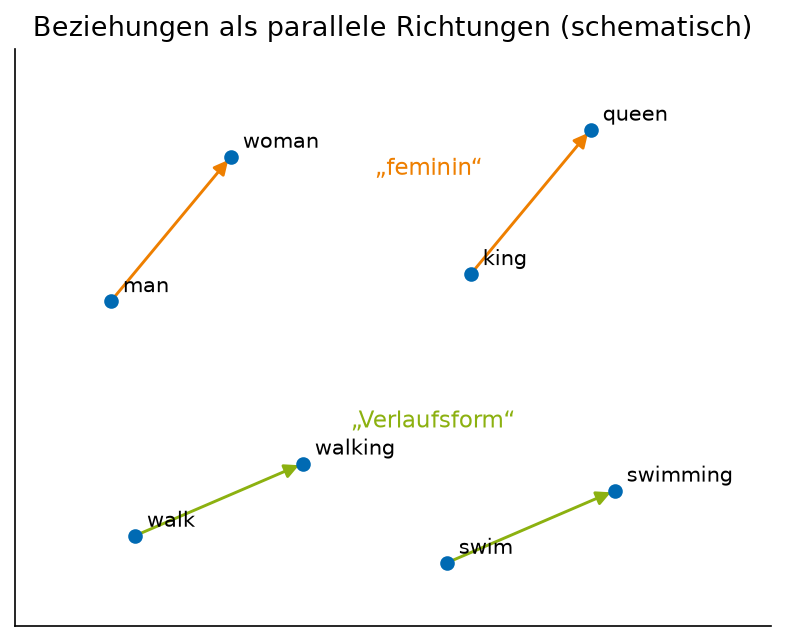
\includegraphics[height=0.6\textheight]{vl13-word-arithmetic.png}
  \end{center}

  \note{Semantische Beziehungen werden zu Richtungen, und Richtungen kann man addieren.
    Das gilt nicht nur für word2vec, sondern für alle LLM-Embeddings -- und ist die
    Grundlage der semantischen Suche, die wir gleich in der Anwendung sehen.}
\end{frame}

\begin{frame}
  \frametitle{Dieselbe Rechnung findet auch das hier}

  \begin{center}
    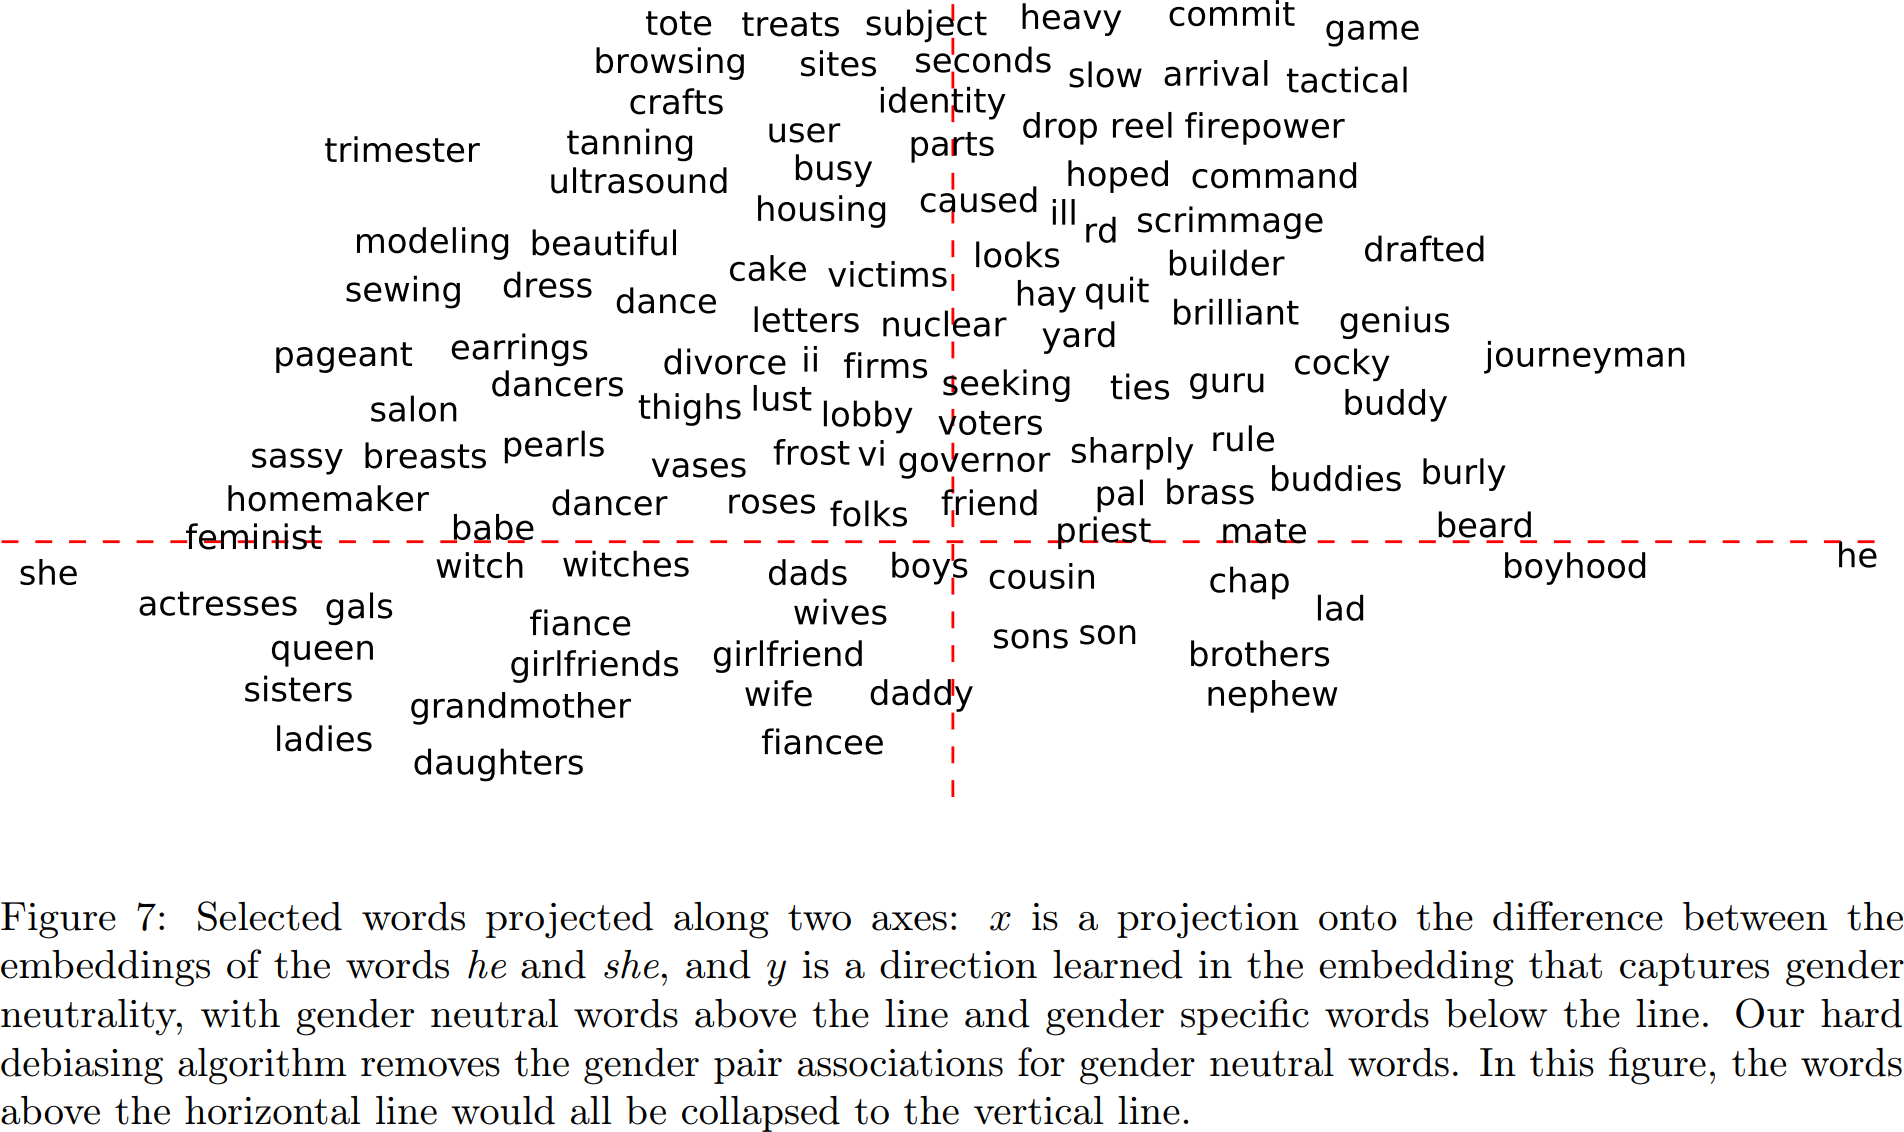
\includegraphics[width=0.52\textwidth]{vl13-bolukbasi-fig7.png}
  \end{center}

  \note{Bolukbasi et al. 2016: \emph{Man is to Computer Programmer as Woman is to
    Homemaker?} Berufe, projiziert auf die Gender-Richtung.
    Die Embeddings enthalten die Stereotype des Trainingskorpus als Richtungen -- und
    weil es Richtungen sind, kann man sie messen und teilweise herausrechnen.
    Das ist eine gute Stelle für zwei Minuten Diskussion: Ist Debiasing die Lösung, oder
    versteckt es nur das Problem?}
\end{frame}

\begin{frame}
  \frametitle{Interpolation und Superposition}

  \begin{center}
    \Large
    $t \cdot \text{Katze} + (1-t)\cdot\text{Hund}$
  \end{center}

  \bigskip
  \begin{center}
    \normalsize Ein Vektor kann mehr ausdrücken als ein Token.
  \end{center}

  \note{Zwischen zwei Token gibt es nichts; zwischen zwei Vektoren gibt es alles.
    Frage in den Raum: Was dekodiert man, wenn man in der Mitte landet? Genau das ist die
    nächste Folie.}
\end{frame}

\begin{frame}
  \frametitle{Interpolation im Bildraum}

  \begin{center}
    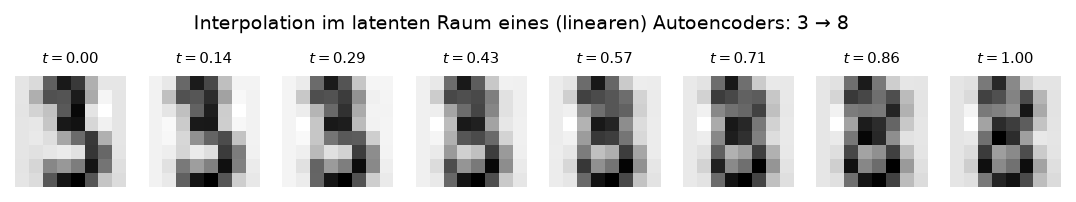
\includegraphics[width=0.78\textwidth]{vl13-latent-interpolation.png}
  \end{center}

  \note{Lineare Interpolation zwischen den Codes einer 3 und einer 8 -- jeder
    Zwischenpunkt ist ein Bild.
    Bei Bildern ist der latente Raum \emph{kontinuierlich}: Jeder Vektor lässt sich
    dekodieren. Bei Text ist das anders -- nächste Folie.}
\end{frame}

\begin{frame}
  \frametitle{Diskreter latenter Raum}

  \begin{center}
    \Large
    Nur $N$ Vektoren im Vokabular sind Token.\\[14pt]
    Was macht man mit allen anderen?
  \end{center}

  \note{Das ist die Frage, die zur Sampling-Strategie führt -- und damit zu dem, was
    ChatGPT tatsächlich tut.
    Antworten sammeln lassen: nächstgelegenes Token nehmen? Das wäre greedy decoding.}
\end{frame}

\begin{frame}
  \frametitle{Vier Wege zu dekodieren}

  \begin{itemize}\setlength{\itemsep}{6pt}
  \item[\textbf{top-1}] nächstes Token (greedy)
  \item[\textbf{sample}] aus der Softmax-Verteilung ziehen
  \item[\textbf{top-$k$}] nur aus den $k$ nächsten ziehen
  \item[\textbf{top-$p$}] so viele, bis die Masse $p$ erreicht ist
  \end{itemize}

  \note{Abstand meist im Kosinus-Abstand.
    Das ist genau die Verteilung, die wir in VL 12 ausgelesen haben -- hier wird
    entschieden, was daraus wird.}
\end{frame}

\begin{frame}
  \frametitle{Temperatur}

  \begin{center}
    \Huge $P_i = \dfrac{\exp(v_i / T)}{\sum_j \exp(v_j / T)}$
  \end{center}

  \bigskip
  \begin{center}
    \normalsize $T > 1$: kreativer. \quad $T < 1$: entschiedener.
  \end{center}

  \note{Die Logits werden durch $T$ geteilt, dann Softmax. Für $T \to 0$ wird daraus
    top-1, für große $T$ die Gleichverteilung.
    Wer den Regler in einer LLM-Oberfläche schon mal gesehen hat: genau der ist gemeint.}
\end{frame}

\begin{frame}
  \frametitle{AE, VAE, GAN nebeneinander}

  \begin{center}
    \Large
    \textbf{AE}: Punkt rein, Punkt raus\\[10pt]
    \textbf{VAE}: Verteilung rein, Prior zieht zusammen\\[10pt]
    \textbf{GAN}: Rauschen rein, Diskriminator als Lehrer
  \end{center}

  \note{Alle drei haben einen latenten Raum, aber mit unterschiedlicher Struktur.
    Beim GAN ist die Verteilung im latenten Raum \emph{vorgegeben} (Standardnormal), beim
    VAE wird sie hingezogen, beim AE ergibt sie sich einfach -- mit Löchern.
    Deshalb kann man aus GAN und VAE sampeln, aus dem AE nur schlecht.}
\end{frame}

\begin{frame}
  \frametitle{Die Geometrie ist krumm}

  \begin{center}
    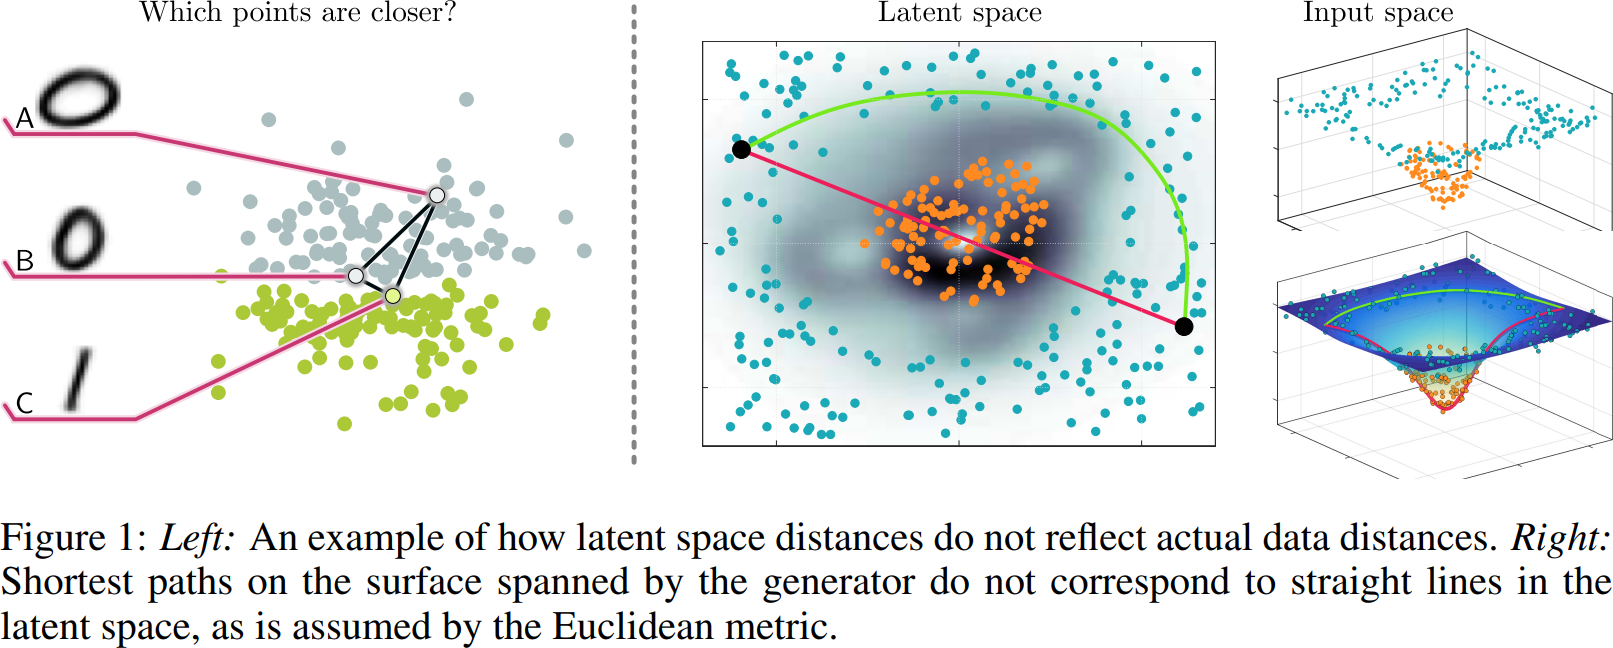
\includegraphics[width=0.66\textwidth]{vl13-arvanitidis-fig1.png}
  \end{center}

  \note{Arvanitidis et al., \emph{Latent Space Oddity} (ICLR 2018): Der latente Raum sieht
    flach aus, aber der Decoder verzerrt ihn. Die euklidische Gerade zwischen zwei Codes
    ist nicht der kürzeste Weg im \emph{Bildraum}.
    \textbf{Take-Home:} Die gerade Linie zwischen zwei Codes läuft oft außerhalb der
    latenten Mannigfaltigkeit -- dann ist es keine Interpolation mehr, sondern
    Extrapolation. Und die können Netze schlecht (VL 7).}
\end{frame}

\begin{frame}
  \frametitle{Was man aus einem latenten Raum herausholt}

  \begin{center}
    \Large
    Nachbarsuche \quad Interpolation \quad Sampling\\[10pt]
    Richtungen mit Bedeutung \quad Clustering
  \end{center}

  \note{Diese Liste ist die Brücke zum Anwendungsteil: Jede der drei Anwendungen gleich
    benutzt genau eine dieser Fähigkeiten.}
\end{frame}

% ------------------------------------------------------------------ Anwendungen
\begin{frame}
  \frametitle{Anwendung 1: hAInrich}

  \begin{center}
    \Large Ein Chatbot, der gar keiner ist.
  \end{center}

  \note{\textbf{Ab hier Dialog, nicht Vortrag.} Die Aufgabe hinschreiben und den Hörsaal
    den Weg vorschlagen lassen; die Folie bestätigt nur.
    Aufgabe: Interface zu einer Wissensdatenbank aus Frage-Antwort-Paaren.
    Erwartete Schritte: FAQ nach JSON, Fragen mit einem LLM in Vektoren (Weg 2 aus VL 12),
    Nutzereingabe ebenso, Kosinus-Ähnlichkeit, Top-3 anzeigen.
    Pointe zum Schluss: Das läuft vollständig im Browser (ONNX, 20 MB Modell) -- kein
    Server sieht die Fragen, also kein Logging-Problem. 2025 hat das 26 Minuten getragen.}
\end{frame}

\begin{frame}
  \frametitle{Anwendung 2: E-Mails klassifizieren}

  \begin{center}
    \Large
    Welche Mail braucht wahrscheinlich eine Antwort?
  \end{center}

  \note{Wieder erst fragen: Woher kommen hier die Label?
    Antwort, auf die man kommen soll: aus dem Ordner „Gesendet“ über den
    \texttt{In-Reply-To}-Header -- wer beantwortet wurde, hat Label 1.
    Dann: IMAP zum Download, Spam ausschließen, Text per LLM in Vektoren, MLP darauf,
    BCE-Loss. Alles Bausteine, die wir haben.}
\end{frame}

\begin{frame}
  \frametitle{Anwendung 3: Empfehlungssystem}

  \begin{center}
    \Large
    Kauflisten sind „Sätze“,\\ Items sind „Wörter“.
  \end{center}

  \note{Das ist die Pointe, auf die der Hörsaal kommen soll: word2vec (Skip-gram) auf
    Kauflisten, oder node2vec auf dem bipartiten Nutzer-Item-Graphen -- beides aus VL 9.
    Danach Nachbarsuche im latenten Raum.
    \textbf{Klausurrelevant:} „Wie trainiert man das Netz für das Empfehlungssystem?“ ist
    genau eine Frage vom Typ Anwendungskonzept.}
\end{frame}

\begin{frame}
  \frametitle{Das Rezept}

  \begin{enumerate}\setlength{\itemsep}{5pt}
  \item Was haben wir? (Daten, Modalität, Label)
  \item Was soll rauskommen? (damit steht die Ausgabeschicht fest)
  \item Welches Modell, und woher? (fast nie von null)
  \item Welcher Loss? (folgt aus 2)
  \item Wie messen wir Güte?
  \end{enumerate}

  \note{Das ist der Aufgabentyp „Anwendungskonzept“ in der Klausur -- und die Struktur,
    die eine gute Antwort haben muss.
    Punkt 3 ist der, an dem die meisten zu viel wollen: ein vortrainiertes Modell
    einfrieren und einen kleinen Kopf trainieren ist fast immer die richtige erste Antwort.
    Nächste Woche: Destillation -- und Vibecoding, also wie man so etwas mit generiertem
    Code tatsächlich baut.}
\end{frame}

\end{document}

%%% Local Variables:
%%% mode: latex
%%% TeX-master: t
%%% End:
